% !TeX root = ../main.tex
% Add the above to each chapter to make compiling the PDF easier in some editors.

\chapter{Base Application}\label{chapter:base_application}

This thesis is focused on optimizing an already existing application. In order to show what optimisations were made, we must first go through the initial application.
This section will focus on the underlying application, while the next will go into the optimisations in detail.\\

\begin{figure}
	\centering
	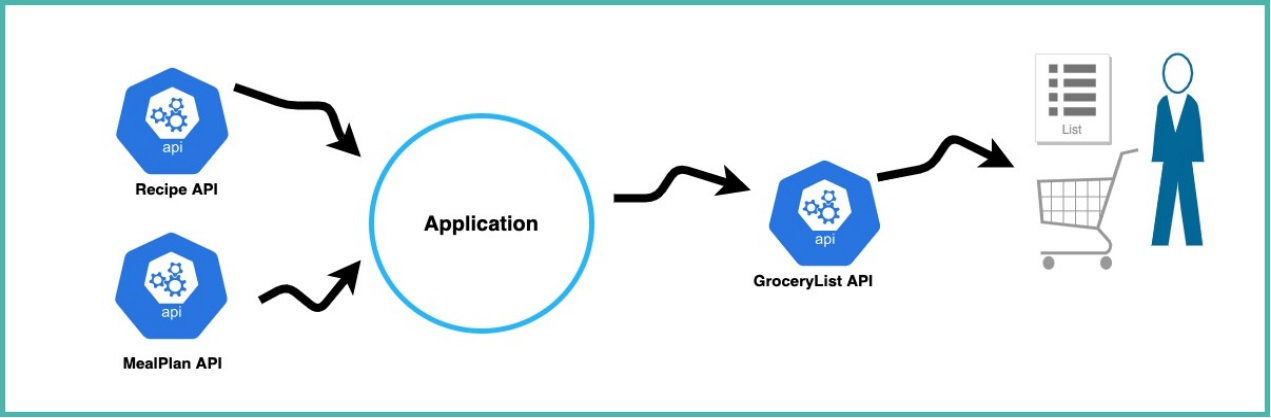
\includegraphics[scale=0.4]{Figures/architecture.jpg}
	\caption[Application Architecture]{High level Architectire of the application}\label{fig:arch}
\end{figure}
The application is API-based, consisting of three APIs: Grocery List API, Recipe API and MealPlan API. The recipe-API manages recipies, their reqired ingredients aswell as the respective quantities and units for them. In addition the individual ingredients are put into categories for the shopping list. For categorisation we use a database provided by the  United States Department of Agracultures, containing around 8800 ingredient-category pairs. On this basis we can vectorise the ingredients, using a pre-trained languge model called BERT. When a new ingredient is added, we vectorise it with BERT. Afterwords we search our vectorspace for the closest vector, matching their category.\\

The MealPlan-API maintains the meal plans. Its main purpose is to map recipies to a stored meal plan. The API maps the recipies for a fixed timeslot aswell as a fixed  number of meals per day.

Finally, in the GroceryList-API we create the shopping list. The GrocerList-API generates the list for a given meal plan and timeslot(in weeks). For the list creation we iterate over each single meal per day for the entire timeframe.
For every meal we iterate over the single ingredients, either increasing the quantity or adding it to the list, if not previously contained. Once the list is complete, we order the list according to a supermarket layout.

